\subsection{集合の圏と射集合}
	圏を定義する際に使用した射集合だが、射集合も集合であるため集合の圏の対象として捉えることができる。射集合というと、未知の集合論的な操作をいくつも持っているのかと考えてしまうが、これから扱う射集合の性質は圏論的に定義されたものだけで事足りる。そのため少し大げさかもしれないが、これから説明する操作や性質を射集合の定義だと考えても良いかもしれない。
  また、ここから一般の圏$\cat{C}$と集合の圏$\cat{Set}$を同時に扱うことになる。そのため、今扱っている対象や射、議論がどの圏上で行われるのかを意識してほしい。

  \begin{define}[共変射写像]
		圏$\cat{C}$の対象$A,B$と射$\mor{f}{A}{B}$に対して、任意の射$\mor{g}{X}{A}$に射$f$を左から合成する写像を
		\begin{align*}
			&\mor{\arset{C}{X}{f}}{\arset{C}{X}{A}}{\arset{C}{X}{B}}\\
			&\arset{C}{X}{f}(g)=f\circ g
		\end{align*}
		\begin{center}
			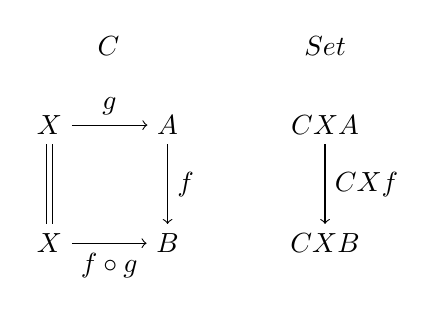
\begin{tikzpicture}[auto]
				\node (x) at (-1.5, 0) {$X$};
				\node (x2) at (-1.5, -1.5) {$X$};
				\node (a) at (0, 0) {$A$};
				\node (b) at (0, -1.5) {$B$};
				\node (ca) at (2, 0) {$\arset{C}{X}{A}$};
				\node (cb) at (2, -1.5) {$\arset{C}{X}{B}$};
				\node (catc) at (-0.75, 1) {$\cat{C}$};
				\node (catc) at (2, 1) {$\cat{Set}$};
				\draw[->] (ca) to node{$\arset{C}{X}{f}$}(cb);
				\draw[->] (a) to node{$f$}(b);
				\draw[double distance=2pt] (x) to (x2);
				\draw[->] (x) to node{$g$}(a);
				\draw[->] (x2) to node[swap]{$f\circ g$}(b);
			\end{tikzpicture}
		\end{center}
		と定義する。またこのような写像を\textbf{共変射写像}と呼ぶことにする。
	\end{define}
  
  圏の定義で確認した射の合成を行う写像\[\mor{\circ}{\arset{C}{A}{B}\times\arset{C}{X}{A}}{\arset{C}{X}{B}}\]
  は、任意の射集合の元の対$\tuple{f,g}$を$f\circ g$に写す写像であったが、共変射写像$\arset{C}{X}{f}$は対の左側の射$f$を固定した写像であることがわかる。

  また射集合の元の対$\tuple{f,g}$は積の普遍性で扱った射の対ではないことに注意してほしい。ただし、条件によっては一対一対応をすることがある。これは後で証明を行う。

  共変射写像では射を左から合成する写像を考えたが、次は射を右から合成する写像である反変射写像を考える。

	\begin{define}[反変射写像]
		圏$\cat{C}$の対象$A,B$と射$\mor{f}{A}{B}$に対して、任意の射$\mor{g}{X}{B}$に射$f$を右から合成する\textbf{反変射写像}を
		\begin{align*}
			&\mor{\arset{C}{f}{X}}{\arset{C}{B}{X}}{\arset{C}{A}{X}}\\
			&\arset{C}{f}{X}(g)=g\circ f
		\end{align*}
		\begin{center}
			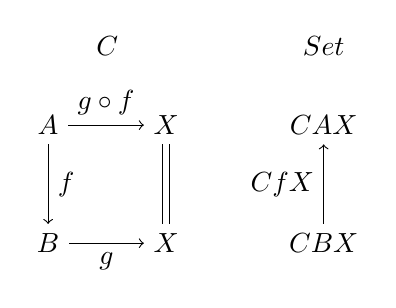
\begin{tikzpicture}[auto]
				\node (x) at (0, 0) {$X$};
				\node (x2) at (0, -1.5) {$X$};
				\node (a) at (-1.5, 0) {$A$};
				\node (b) at (-1.5, -1.5) {$B$};
				\node (ca) at (2, 0) {$\arset{C}{A}{X}$};
				\node (cb) at (2, -1.5) {$\arset{C}{B}{X}$};
				\node (catc) at (-0.75, 1) {$\cat{C}$};
				\node (catc) at (2, 1) {$\cat{Set}$};
				\draw[->] (cb) to node{$\arset{C}{f}{X}$}(ca);
				\draw[->] (a) to node{$f$}(b);
				\draw[double distance=2pt] (x) to (x2);
				\draw[->] (a) to node{$g\circ f$}(x);
				\draw[->] (b) to node[swap]{$g$}(x2);
			\end{tikzpicture}
		\end{center}
		と定義する。共変射写像と違い、射$f$に対して$\arset{C}{f}{X}$の向きが逆になっている。
	\end{define}

  これまでは一般の圏$\cat{C}$の射集合についての議論を行なってきたが、以降は射集合を取る圏を$\cat{Set}$に限定して行うことにする。理由としては$\cat{Set}$上の射集合もまた集合であり、$\cat{Set}$の対象であるためである。そのため、射集合とその始域、終域となる集合の間に射を伸ばすことができ、射集合のさらなる性質を記述することができるようになる。

  次に射写像の応用として、対象の同型との関係性を見る。

  \begin{prop}[同型射となる共変射写像]ある圏$\cat{C}$において$B\cong B'\Longrightarrow$任意の対象$X$に対し$\arset{C}{X}{B}\cong\arset{C}{X}{B'}$
  \end{prop}

  \begin{proof}
    同型射を$\mor{i}{B}{B'}$、$\mor{i^{-1}}{B'}{B}$として、共変射写像\[\mor{\arset{C}{X}{i}}{\arset{C}{X}{B}}{\arset{C}{X}{B'}}\]と\[\mor{\arset{C}{X}{i^{-1}}}{\arset{C}{X}{B'}}{\arset{C}{X}{B}}\]もまた同型射になることを示す。すなわち、\[\arset{C}{X}{i}\circ\arset{C}{X}{i^{-1}}=id_{\arset{C}{X}{B'}}\]\[\arset{C}{X}{i^{-1}}\circ\arset{C}{X}{i}=id_{\arset{C}{X}{B}}\]を示せばよい。

    射集合$\arset{C}{X}{B'}$の任意の元$\mor{f}{X}{B'}$に対して、
    \begin{align*}
      \arset{C}{X}{i}\circ\arset{C}{X}{i^{-1}}(f)&=\arset{C}{X}{i}(\arset{C}{X}{i^{-1}}(f))&\text{(写像の合成の定義)}\\
      &=\arset{C}{X}{i}(i^{-1}\circ f)&\text{(共変射写像の定義)}\\
      &=i\circ i^{-1}\circ f&\text{(共変射写像の定義)}\\
      &=id_{B'}\circ f&\text{(同型射の定義)}\\
      &=f&\text{(恒等射の定義)}\\
      &=id_{\arset{C}{X}{B'}}(f)&\text{(恒等射の定義)}
    \end{align*}
    よって$\arset{C}{X}{i}\circ\arset{C}{X}{i^{-1}}=id_{\arset{C}{X}{B'}}$が示せた。同様に$\arset{C}{X}{i^{-1}}\circ\arset{C}{X}{i}=id_{\arset{C}{X}{B}}$も示せる。
    
    よって$\mor{\arset{C}{X}{i}}{\arset{C}{X}{B}}{\arset{C}{X}{B'}}$と$\mor{\arset{C}{X}{i^{-1}}}{\arset{C}{X}{B'}}{\arset{C}{X}{B}}$もまた同型射となるため、$\arset{C}{X}{B}\cong\arset{C}{X}{B'}$が成り立つ。
		\begin{center}
			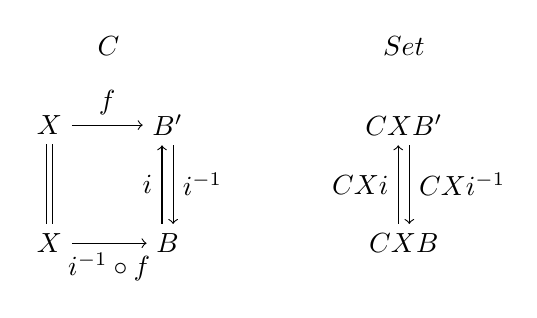
\begin{tikzpicture}[auto]
				\node (x) at (-1.5, 0) {$X$};
				\node (x2) at (-1.5, -1.5) {$X$};
				\node (a) at (0, -1.5) {$B$};
				\node (b) at (0, 0) {$B'$};
				\node (ca) at (3, -1.5) {$\arset{C}{X}{B}$};
				\node (cb) at (3, 0) {$\arset{C}{X}{B'}$};
				\node (catc) at (-0.75, 1) {$\cat{C}$};
				\node (catc) at (3, 1) {$\cat{Set}$};
				\draw[->,transform canvas={xshift=-2pt}] (ca) to node{$\arset{C}{X}{i}$}(cb);
        \draw[->,transform canvas={xshift=2pt}] (cb) to node{$\arset{C}{X}{i^{-1}}$}(ca);
				\draw[->,transform canvas={xshift=-2pt}] (a) to node{$i$}(b);
        \draw[->,transform canvas={xshift=2pt}] (b) to node{$i^{-1}$}(a);

				\draw[double distance=2pt] (x) to (x2);
				\draw[->] (x2) to node[swap]{$i^{-1}\circ f$}(a);
				\draw[->] (x) to node{$f$}(b);
			\end{tikzpicture}
		\end{center}
  \end{proof}
  
  また同様の性質が反変射写像でも成り立つ
  \begin{prop}[同型射となる反変射写像]
    ある圏$\cat{C}$において$A\cong A'\iff$任意の対象$X$に対し$\arset{C}{A}{X}\cong\arset{C}{A'}{X}$
  \end{prop}

  一つ前の命題の任意の対象$X$に終対象$1$を当てはめると、\[B\cong B'\Longrightarrow \arset{C}{1}{B}\cong\arset{C}{1}{B'}\]となる。$\arset{C}{1}{B}$は$B$の元の集合である。それらが同型であるということは、$B$の元と$B'$の元が一対一対応をするということであり、前に示した元と同型の関係性そのものであることが分かる。\\
  さらに任意の対象$X$に拡張することで、元$\mor{b}{1}{B}$が一対一対応をするだけでなく、射$\mor{f}{X}{B}$までもが一対一対応をすることが分かった。射の対応も元と同様に$f\sim f'$と表すことにする。
  \begin{define}[評価射]
		集合の圏$\cat{Set}$の任意の対象$A,B$と$B$の元$b$、$\cat{Set}$の射$\mor{f}{B}{A}$に対して\textbf{評価射}を
		\begin{align*}
			\mor{&ev_{A,B}}{\arset{Set}{B}{A}\times B}{A}\\
			&ev_{A,B}(\tuple{f,b})=f(b)\\
		\end{align*}
		と定義する。もしくは
    これは元$b$に写像$f$を適用する操作を写像にしたものである。またこのような射は任意の対象$A,B$に対して個別に存在するが、現段階では添え字としての対象を省略し、特に区別はしない。
		厳密な証明は行わないが評価射は実際に写像になる。
	\end{define}

	\begin{define}[余評価射]
		集合の圏$\cat{Set}$の任意の対象$A,B$と$A$の元$a$に対して\textbf{余評価射}を
		\begin{align*}
			\mor{&ce_{A,B}}{A}{\arset{Set}{B}{A\times B}}\\
			&ce_{A,B}(a)=\lambda x.\tuple{a,x}\mor{}{B}{A\times B}\\
			&\lambda x.\tuple{a,x}(b)=\tuple{a,b}
		\end{align*}
		と定義する。また\[ce_{A,B}(a)(b)=\tuple{a,b}\]とも表記できる。
    同様にこのような射は任意の対象$A,B$に対して個別に存在するが区別しない。
	\end{define}

  また、余評価射によって得られる射$\mor{\lambda x.\tuple{a,x}}{B}{A\times B}$と任意の射$\mor{f}{C}{B}$、$\mor{g}{A\times B}{C}$との合成に対して以下の表記を導入する。
  \begin{center}
    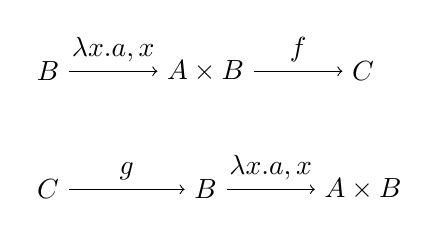
\begin{tikzpicture}[auto]
      \node (c) at (0, 0) {$C$};
      \node (b) at (2, 0) {$B$};
      \node (ab) at (4, 0) {$A\times B$};
      \draw[->] (c) to node{$g$}(b);
      \draw[->] (b) to node{$\lambda x.\tuple{a,x}$}(ab);

      \node (b) at (0, 1.5) {$B$};
      \node (ab) at (2, 1.5) {$A\times B$};
      \node (c) at (4, 1.5) {$C$};
      \draw[->] (b) to node{$\lambda x.\tuple{a,x}$}(ab);
      \draw[->] (ab) to node{$f$}(c);
    \end{tikzpicture}
  \end{center}
  \begin{align*}
    (\lambda x.\tuple{a,x})\circ f &=\lambda x.\tuple{a,f(x)}\\
    g\circ(\lambda x.\tuple{a,x}) &=\lambda x.g(\tuple{a,x})
  \end{align*}

  定義からわかるように、$B$の任意の値$b$を適用すると、
  \begin{align*}
    \lambda x.\tuple{a,f(x)}(b)&=\tuple{a,f(b)}\\
    \lambda x.g(\tuple{a,x})(b)&=g(\tuple{a,b})
  \end{align*}
  となる。
  余評価射の定義に値の適用を用いたが、これは評価射で表すことができる。次はこのような評価射と余評価射の関係性、性質を見ていく。以下証明する二つの命題は当分使用しないため、興味がなければ飛ばしてもらっても構わない。

  \begin{prop}[冪の三角恒等式1]
    任意の対象$A,B$において、\[ce\circ \arset{Set}{B}{ev}=id_{\arset{Set}{B}{A}}\]が成り立つ。
    \begin{center}
			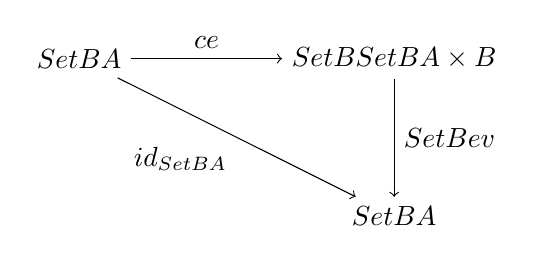
\begin{tikzpicture}[auto]
				\node (setba1) at (0, 0) {$\arset{Set}{B}{A}$};
        \node (setbbab) at (4, 0) {$\arset{Set}{B}{\arset{Set}{B}{A}\times B}$};
				\node (setba2) at (4, -2) {$\arset{Set}{B}{A}$};

				\draw[->] (setba1) to node[swap]{$id_{\arset{Set}{B}{A}}$}
        (setba2);
        \draw[->] (setba1) to node{$ce$}(setbbab);
        \draw[->] (setbbab) to node{$\arset{Set}{B}{ev}$}(setba2);
			\end{tikzpicture}
		\end{center}
  \end{prop}

  \begin{proof}
    任意の射$\mor{f}{B}{A}$に対して、
    \begin{align*}
      \arset{Set}{B}{ev}\circ ce(f)&=\arset{Set}{B}{ev}(\lambda x.\tuple{f,x})&\text{(余評価射の定義)}\\
      &=ev\circ\lambda x.\tuple{f,x}&\text{(共変射写像の定義)}\\
      &=\lambda x.ev(\tuple{f,x})\\
      &=\lambda x.f(x)&\text{(評価射の定義)}
    \end{align*}
    となる。直感的に明らかではあるが、$\lambda x.f(x)=f$を示す。
    対象$B$の任意の元$b$に対して余評価射の定義から\[(\lambda x.f(x))(b)=f(b)\]となる。よって\[\lambda x.f(x)=f\]となり、これが任意の射$f$で成り立つから、
    \[ce\circ \arset{Set}{B}{ev}=id_{\arset{Set}{B}{A}}\]となる。
  \end{proof}

  \begin{prop}[冪の三角恒等式2]
    任意の対象$A,B$において、\[ev\circ(ce\times id_B)=id_{A\times B}\]が成り立つ。
    \begin{center}
			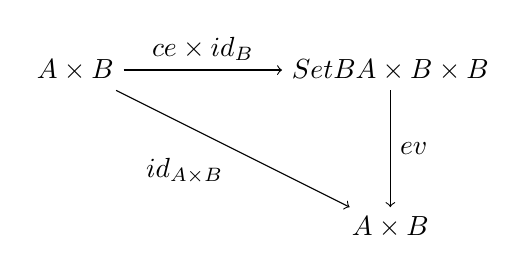
\begin{tikzpicture}[auto]
				\node (setba1) at (0, 0) {$A\times B$};
        \node (setbbab) at (4, 0) {$\arset{Set}{B}{A\times B}\times B$};
				\node (setba2) at (4, -2) {$A\times B$};

				\draw[->] (setba1) to node[swap]{$id_{A\times B}$}
        (setba2);
        \draw[->] (setba1) to node{$ce\times id_B$}(setbbab);
        \draw[->] (setbbab) to node{$ev$}(setba2);
			\end{tikzpicture}
		\end{center}
  \end{prop}

  \begin{proof}
    対象$A\times B$の任意の元$\tuple{a,b}$に対して、
    \begin{align*}
      ev\circ (ce\times id_B)(\tuple{a,b})
      &=ev(\tuple{ce(a),b})&\text{(射の積の定義)}\\
      &=ev(\tuple{\lambda x.\tuple{a,x},b})&\text{(余評価射の定義)}\\
      &=\lambda x.\tuple{a,x}(b)&\text{(評価射の定義)}\\
      &=\tuple{a,b}&\text{(余評価射の定義)}
    \end{align*}
    となる。よって\[ev\circ(ce\times id_B)=id_{A\times B}\]が成り立つ。
  \end{proof}
